\documentclass[english, 11 pt, class=article, crop=false]{standalone}
\usepackage[T1]{fontenc}
%\renewcommand*\familydefault{\sfdefault} % For dyslexia-friendly text
\usepackage{lmodern} % load a font with all the characters
\usepackage{geometry}
\geometry{verbose,paperwidth=16.1 cm, paperheight=24 cm, inner=2.3cm, outer=1.8 cm, bmargin=2cm, tmargin=1.8cm}
\setlength{\parindent}{0bp}
\usepackage{import}
\usepackage[subpreambles=false]{standalone}
\usepackage{amsmath}
\usepackage{amssymb}
\usepackage{esint}
\usepackage{babel}
\usepackage{tabu}
\makeatother
\makeatletter

\usepackage{titlesec}
\usepackage{ragged2e}
\RaggedRight
\raggedbottom
\frenchspacing

% Norwegian names of figures, chapters, parts and content
\addto\captionsenglish{\renewcommand{\figurename}{Figur}}
\makeatletter
\addto\captionsenglish{\renewcommand{\chaptername}{Kapittel}}
\addto\captionsenglish{\renewcommand{\partname}{Del}}


\usepackage{graphicx}
\usepackage{float}
\usepackage{subfig}
\usepackage{placeins}
\usepackage{cancel}
\usepackage{framed}
\usepackage{wrapfig}
\usepackage[subfigure]{tocloft}
\usepackage[font=footnotesize,labelfont=sl]{caption} % Figure caption
\usepackage{bm}
\usepackage[dvipsnames, table]{xcolor}
\definecolor{shadecolor}{rgb}{0.105469, 0.613281, 1}
\colorlet{shadecolor}{Emerald!15} 
\usepackage{icomma}
\makeatother
\usepackage[many]{tcolorbox}
\usepackage{multicol}
\usepackage{stackengine}

\usepackage{esvect} %For vectors with capital letters

% For tabular
\usepackage{array}
\usepackage{multirow}
\usepackage{longtable} %breakable table

% Ligningsreferanser
\usepackage{mathtools}
\mathtoolsset{showonlyrefs}

% index
\usepackage{imakeidx}
\makeindex[title=Indeks]

%Footnote:
\usepackage[bottom, hang, flushmargin]{footmisc}
\usepackage{perpage} 
\MakePerPage{footnote}
\addtolength{\footnotesep}{2mm}
\renewcommand{\thefootnote}{\arabic{footnote}}
\renewcommand\footnoterule{\rule{\linewidth}{0.4pt}}
\renewcommand{\thempfootnote}{\arabic{mpfootnote}}

%colors
\definecolor{c1}{cmyk}{0,0.5,1,0}
\definecolor{c2}{cmyk}{1,0.25,1,0}
\definecolor{n3}{cmyk}{1,0.,1,0}
\definecolor{neg}{cmyk}{1,0.,0.,0}

% Lister med bokstavar
\usepackage[inline]{enumitem}

\newcounter{rg}
\numberwithin{rg}{chapter}
\newcommand{\reg}[2][]{\begin{tcolorbox}[boxrule=0.3 mm,arc=0mm,colback=blue!3] {\refstepcounter{rg}\phantomsection \large \textbf{\therg \;#1} \vspace{5 pt}}\newline #2  \end{tcolorbox}\vspace{-5pt}}

\newcommand\alg[1]{\begin{align} #1 \end{align}}

\newcommand\eks[2][]{\begin{tcolorbox}[boxrule=0.3 mm,arc=0mm,enhanced jigsaw,breakable,colback=green!3] {\large \textbf{Eksempel #1} \vspace{5 pt}\\} #2 \end{tcolorbox}\vspace{-5pt} }

\newcommand{\st}[1]{\begin{tcolorbox}[boxrule=0.0 mm,arc=0mm,enhanced jigsaw,breakable,colback=yellow!12]{ #1} \end{tcolorbox}}

\newcommand{\spr}[1]{\begin{tcolorbox}[boxrule=0.3 mm,arc=0mm,enhanced jigsaw,breakable,colback=yellow!7] {\large \textbf{Språkboksen} \vspace{5 pt}\\} #1 \end{tcolorbox}\vspace{-5pt} }

\newcommand{\sym}[1]{\colorbox{blue!15}{#1}}

\newcommand{\info}[2]{\begin{tcolorbox}[boxrule=0.3 mm,arc=0mm,enhanced jigsaw,breakable,colback=cyan!6] {\large \textbf{#1} \vspace{5 pt}\\} #2 \end{tcolorbox}\vspace{-5pt} }

\newcommand\algv[1]{\vspace{-11 pt}\begin{align*} #1 \end{align*}}

\newcommand{\regv}{\vspace{5pt}}
\newcommand{\mer}{\textsl{Merk}: }
\newcommand{\mers}[1]{{\footnotesize \mer #1}}
\newcommand\vsk{\vspace{11pt}}
\newcommand\vs{\vspace{-11pt}}
\newcommand\vsb{\vspace{-16pt}}
\newcommand\sv{\vsk \textbf{Svar} \vspace{4 pt}\\}
\newcommand\br{\\[5 pt]}
\newcommand{\figp}[1]{../fig/#1}
\newcommand\algvv[1]{\vs\vs\begin{align*} #1 \end{align*}}
\newcommand{\y}[1]{$ {#1} $}
\newcommand{\os}{\\[5 pt]}
\newcommand{\prbxl}[2]{
\parbox[l][][l]{#1\linewidth}{#2
	}}
\newcommand{\prbxr}[2]{\parbox[r][][l]{#1\linewidth}{
		\setlength{\abovedisplayskip}{5pt}
		\setlength{\belowdisplayskip}{5pt}	
		\setlength{\abovedisplayshortskip}{0pt}
		\setlength{\belowdisplayshortskip}{0pt} 
		\begin{shaded}
			\footnotesize	#2 \end{shaded}}}

\renewcommand{\cfttoctitlefont}{\Large\bfseries}
\setlength{\cftaftertoctitleskip}{0 pt}
\setlength{\cftbeforetoctitleskip}{0 pt}

\newcommand{\bs}{\\[3pt]}
\newcommand{\vn}{\\[6pt]}
\newcommand{\fig}[1]{\begin{figure}
		\centering
		\includegraphics[]{\figp{#1}}
\end{figure}}

\newcommand{\figc}[2]{\begin{figure}
		\centering
		\includegraphics[]{\figp{#1}}
		\caption{#2}
\end{figure}}

\newcommand{\sectionbreak}{\clearpage} % New page on each section

\newcommand{\nn}[1]{
\begin{equation}
	#1
\end{equation}
}

% Equation comments
\newcommand{\cm}[1]{\llap{\color{blue} #1}}

\newcommand\fork[2]{\begin{tcolorbox}[boxrule=0.3 mm,arc=0mm,enhanced jigsaw,breakable,colback=yellow!7] {\large \textbf{#1 (forklaring)} \vspace{5 pt}\\} #2 \end{tcolorbox}\vspace{-5pt} }
 
%colors
\newcommand{\colr}[1]{{\color{red} #1}}
\newcommand{\colb}[1]{{\color{blue} #1}}
\newcommand{\colo}[1]{{\color{orange} #1}}
\newcommand{\colc}[1]{{\color{cyan} #1}}
\definecolor{projectgreen}{cmyk}{100,0,100,0}
\newcommand{\colg}[1]{{\color{projectgreen} #1}}

% Methods
\newcommand{\metode}[2]{
	\textsl{#1} \\[-8pt]
	\rule{#2}{0.75pt}
}

%Opg
\newcommand{\abc}[1]{
	\begin{enumerate}[label=\alph*),leftmargin=18pt]
		#1
	\end{enumerate}
}
\newcommand{\abcs}[2]{
	\begin{enumerate}[label=\alph*),start=#1,leftmargin=18pt]
		#2
	\end{enumerate}
}
\newcommand{\abcn}[1]{
	\begin{enumerate}[label=\arabic*),leftmargin=18pt]
		#1
	\end{enumerate}
}
\newcommand{\abch}[1]{
	\hspace{-2pt}	\begin{enumerate*}[label=\alph*), itemjoin=\hspace{1cm}]
		#1
	\end{enumerate*}
}
\newcommand{\abchs}[2]{
	\hspace{-2pt}	\begin{enumerate*}[label=\alph*), itemjoin=\hspace{1cm}, start=#1]
		#2
	\end{enumerate*}
}

% Oppgaver
\newcommand{\opgt}{\phantomsection \addcontentsline{toc}{section}{Oppgaver} \section*{Oppgaver for kapittel \thechapter}\vs \setcounter{section}{1}}
\newcounter{opg}
\numberwithin{opg}{section}
\newcommand{\op}[1]{\vspace{15pt} \refstepcounter{opg}\large \textbf{\color{blue}\theopg} \vspace{2 pt} \label{#1} \\}
\newcommand{\ekspop}[1]{\vsk\textbf{Gruble \thechapter.#1}\vspace{2 pt} \\}
\newcommand{\nes}{\stepcounter{section}
	\setcounter{opg}{0}}
\newcommand{\opr}[1]{\vspace{3pt}\textbf{\ref{#1}}}
\newcommand{\oeks}[1]{\begin{tcolorbox}[boxrule=0.3 mm,arc=0mm,colback=white]
		\textit{Eksempel: } #1	  
\end{tcolorbox}}
\newcommand\opgeks[2][]{\begin{tcolorbox}[boxrule=0.1 mm,arc=0mm,enhanced jigsaw,breakable,colback=white] {\footnotesize \textbf{Eksempel #1} \\} \footnotesize #2 \end{tcolorbox}\vspace{-5pt} }
\newcommand{\rknut}{
Rekn ut.
}

%License
\newcommand{\lic}{\textit{Matematikken sine byggesteinar by Sindre Sogge Heggen is licensed under CC BY-NC-SA 4.0. To view a copy of this license, visit\\ 
		\net{http://creativecommons.org/licenses/by-nc-sa/4.0/}{http://creativecommons.org/licenses/by-nc-sa/4.0/}}}

%referances
\newcommand{\net}[2]{{\color{blue}\href{#1}{#2}}}
\newcommand{\hrs}[2]{\hyperref[#1]{\color{blue}\textsl{#2 \ref*{#1}}}}
\newcommand{\rref}[1]{\hrs{#1}{regel}}
\newcommand{\refkap}[1]{\hrs{#1}{kapittel}}
\newcommand{\refsec}[1]{\hrs{#1}{seksjon}}

\newcommand{\mb}{\net{https://sindrsh.github.io/FirstPrinciplesOfMath/}{MB}}


%line to seperate examples
\newcommand{\linje}{\rule{\linewidth}{1pt} }

\usepackage{datetime2}
%%\usepackage{sansmathfonts} for dyslexia-friendly math
\usepackage[]{hyperref}


\begin{document}

\opgt
\setcounter{section}{1}	
\op{udir}
Utdanninsdirektoratet definerer størrelsen til en vinkel $ v $ mellom to linjestykker $ a $ og $ b $, oppgitt i radianer,  på følgende måte:\os

\textsl{Forholdet mellom lengden på en bue mellom $ a $ og $ b $ og radiusen til buen.}
\begin{figure}
	\centering
	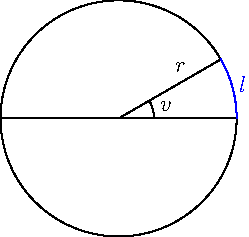
\includegraphics[]{../../fig/rad}
\end{figure}
I figuren over svarer dette til forholdet $ \dfrac{l}{r} $.
\os
Forklar hvorfor radianer ut ifra denne definisjonen også kan sees på som en buelengde langs enhetssirkelen.

\op{rads}
Gjør om til radianer:\os
\begin{tabular}{@{}l l}
	\textbf{a)} $ 60^\circ $ & \quad \textbf{b)} $ 15^\circ $
\end{tabular}

\op{grad}
Gjør om til grader:\os

\begin{tabular}{@{}l l}
	\textbf{a)} $ \dfrac{11\pi}{12} $ & \quad \textbf{b)} $ \dfrac{11\pi}{6} $
\end{tabular}

\nes
\op{pytg}
Bruk Pytagoras' setning og definisjonen av $ \cos x $ og $ \sin x $ til å vise at
\[ \cos^2 x + \sin^2 x = 1 \] 

\op{tanx}
Finn $\tan x $ når du vet at\\
\begin{tabular}{@{}l l}
	\textbf{a)} $ \sin x = 0$ og $ \cos x=1 $ & \quad \textbf{b)} $ \sin x = \dfrac{1}{2} $ og $ \cos x = -\dfrac{\sqrt{3}}{2} $
\end{tabular}
\newpage
\op{kvadrant}
Bruk $ - $ og $ + $ for å indikere henholdsvis negativ og positiv, og sett riktige markører i tabellen under.\os

\begin{tabular}{@{}l|l| l| l|l|}
&1. kvadrant & 2. kvadrant & 3. kvadrant & 4. kvadrant\\ \hline
$ \sin x $& & & &\\ \hline
$ \cos x $& & & &\\ \hline
$ \tan x $& & & &\\\hline
\end{tabular}

\op{trigverd}
Bestem verdien til\os
\begin{tabular}{@{}l l l l }
\textbf{a)} $ \sin\left(-\frac{\pi}{6}\right) $ &\quad \textbf{b)} $ \cos \pi $ &\quad \textbf{c)} $ \cos\left(-\frac{\pi}{2}\right) $&\quad \textbf{d)} $ \tan\left(\frac{2\pi}{3}\right) $
\end{tabular}

\op{averdier}
Finn verdien til\\ \renewcommand{\arraystretch}{1.7}
\begin{tabular}{@{}l l l l }	
\textbf{a)} $ \asin 0 $ &\quad\textbf{b)} $ \asin \frac{\sqrt{3}}{2} $ \\
 \textbf{c)} $ \acos (-1) $ &\quad\textbf{d)} $ \acos \left(-\frac{\sqrt{2}}{2}\right) $ \\
 \textbf{e)} $ \atan 1 $ &\quad\textbf{f)} $ \atan \left(\frac{1}{\sqrt{3}}\right) $
\end{tabular}\renewcommand{\arraystretch}{1}

\op{bruk1}
Bruk \eqref{1} til å vise at $ {\sin\left(\frac{\pi}{6}\right)=\frac{1}{2}} $ når du vet at $ \cos\left(\frac{\pi}{6}\right)=\frac{\sqrt{3}}{2} $.

\op{sin2xopg}
\textbf{a)} Bruk én av de trigonometriske identitetene til å vise at
\[  \sin (2x)=2\cos x\sin x \]
\textbf{b)} Gitt at $ {\sin \left(\frac{\pi}{6}\right)=\frac{1}{2}} $. Bruk dette og identiteten over til å vise at
\[ 2\cos \left(\frac{\pi}{12}\right)\sin \left(\frac{\pi}{12}\right) = \frac{1}{2} \]

\op{cossomsin}
Skriv om utrykket
\[ \cos \left(3x-\frac{5\pi}{2}\right) \]
til et sinusuttrykk.
\newpage
\op{cossinsin}
Skriv om uttrykket \[ \cos( 2x) + \sqrt 3\sin (2x) \]
til et sinusuttrykk.

\nes

\op{sincos0}
Vis at alle løsninger av ligningen $ \cos x=0 $ er gitt som
\[ x = \frac{\pi}{2}+\pi n \]
mens alle løsninger av ligningen $ \sin x = 0 $ er gitt som
\[ x = \pi n \]\vs \vs

\op{triligns}
Løs ligningene:\os

\textbf{a)} $ \cos x=\frac{\sqrt{2}}{2} $\os

\textbf{b)} $ \cos \left(\frac{\pi}{3}x\right) = 0\quad,\quad x\in[0, 5]$\os

\textbf{c)} $ 2\sin(3x)=1 $\os

\textbf{d)} $ \sin(2x-\pi)=-\frac{\sqrt{3}}{2} $\os

\textbf{e)} $ 2\sqrt{3}\tan \left(4x+\frac{\pi}{2}\right) = 2$ \os

\op{asinbcos0o}
Løs ligningene:\os

\textbf{a)} $\sqrt{3} \sin x - \cos x =0$\os

\textbf{b)} $ \sin x + \sqrt{3}\cos x =0$\os

\textbf{c)} $ \cos (2x) + \sin (2x)=0  $\os


\op{kombo}
Løs ligningene:\os
\textbf{a)} $ \cos x - \sin x = \sqrt{2}  $ \os

\textbf{b)} $ \sqrt{3} \cos\left(\dfrac{x}{2\pi}\right) - \sin\left(\dfrac{x}{2\pi}\right)=1 $\os
\nes
\newpage
\op{abctri}
Løs ligningene:\os
\textbf{a)} $ \sin^2 x+\frac{1}{2}\sin x-\frac{1}{2}=0 $\os

\textbf{b)} $ \cos^2 (3x) -3\cos (3x) -4=0$\os

\textbf{c)} $ 2\cos^2 x+ \sqrt{8} \cos x+1=0 $\os

\textbf{d)} $ \tan^2 (\pi x) -\sqrt{12}\tan (\pi x) +  3=0$\os

\textbf{e)} $ -\sin^2(3x)- 3\cos (3x) -3=0$ \os


\op{kvadopg} 
Løs ligningene:\os

\textbf{a)} $ -\cos^2 x+15\sin^2 x = 3 $ 

\textbf{b)} $ \cos^2 \left(\dfrac{x}{4}\right) - 2 \sin^2 \left(\dfrac{x}{4}\right) = -\dfrac{1}{2} $

\nes
\op{cosmaks}	
Forklar hvorfor en cosinusfunksjon $ f(x)=a\cos(kx+c)+d $ har\os

\textbf{a)} Maksimalverdier for $ kx+c= 2\pi n$ og minimalverdier for $ kx+c= \pi + 2\pi n $ når $ a>0 $.\os

\textbf{b)} Maksimalverdier for $ kx+c= \pi+2\pi n$ og minimalverdier for $ kx+c= 2\pi n $ når $ a<0 $. 

\op{cosfunko}
Gitt funksjonen 
\[ f(x)=-3\cos\left(3x+\frac{\pi}{12}\right)+4 \]
\textbf{a)} Finn perioden til $ f $.\os

\textbf{b)} Hva er minimums- og maksimumsverdiene til $ f $?\os

\textbf{c)} Finn alle $ x $ hvor $ f $ har minimums- og maksimumsverdier.


\op{sinmaks}
Forklar hvorfor en sinusfunksjon $ f(x)=a\sin(kx+c)+d $ har\os

\textbf{a)} Maksimalverdier for $ kx+c=\dfrac{\pi}{2}+ 2\pi n$ og minimalverdier for $ kx+c= -\dfrac{\pi}{2} + 2\pi n $ når $ a>0 $.\os

\textbf{b)} Maksimalverdier for $ kx= \pi+2\pi n$ og minimalverdier for $ kx= 2\pi n $ når $ a<0 $. 
\newpage
\op{sinfnpkt}
Gitt funksjonen 
\[ f(x)=-2\sin\left(\frac{\pi}{2}x\right)+1 \quad, \quad x\in[-5, 5]\]
\textbf{a)} Finn perioden til $ f $.\os

\textbf{b)} Finn topppunktene til $ f $. \os

\textbf{c)} Finn nullpunktene til $ f $.\os

\op{skissin}
Om en cosinusfunksjon vet du følgende:
\begin{itemize}
	\item likevektslinja til funksjonen er $ y=1 $.
	\item $ (0,3) $ og $ (2\pi, 3) $ er to naboliggende toppunkt.
\end{itemize}
Skisser grafen til funksjonen for ${ x\in[0, 3\pi]} $.

\op{sincosfig}
\vspace{-10 pt}
\subimport{../../tri/fig/}{cosopg2}
\vs
\textbf{a)} Finn et cosinusuttrykk til grafen over.\os

\textbf{b)} Finn et sinusuttrykk til grafen over.


\op{tanfopg}
Forklar hvorfor alle funksjoner $ f $ på formen
\[ f(x)= a \tan (kx+c)+d\]
har vertikale figr når
\[ kx+c=\pm \frac{\pi}{2}+\pi n \]
\newpage
\grubop{opgtangr}
Gitt at
\[ \tan x = \frac{a}{b} \]
Vis at $ \sin x = \dfrac{a}{\sqrt{a^2+b^2}} $ og at $ \cos x = \dfrac{b}{\sqrt{a^2+b^2}} $.
\begin{comment}


\ekspop
I denne oppgaven skal vi komme fram til to viktige resultater, nemlig at:
\alg{
\lim\limits_{x\to 0}\frac{\sin x}{x}&=1 \\ &\\
\lim\limits_{x\to 0}\frac{\cos x-1}{x}&=0 	
}
Når vi i \textsl{Kapittel 6} finner den deriverte av $ \sin x $ og $ \cos x $, brukes blant annet disse resultatene.
\begin{figure}[H]
\centering
\includegraphics[]{\asym{sinx}}
\end{figure}
a) Bruk formlikhet til å vise at $ \tan x $ er høyden i figuren over.

b) Forklar hvorfor vi må ha at:
\[ \frac{\sin x}{x}<1 \]
c) Buen $ x $ utgjør $ \frac{x}{2\pi} $ av omkretsen til enhetssirkelen. Vis at arealet av sektoren til $ x $ blir $ \frac{1}{2}x $.

d) Forklar hvorfor vi må ha at:
\alg{
\frac{1}{2}x&<\frac{1}{2}\tan x	\\
x&<\tan x	
}
e) Bruk ulikhetene fra \textsl{b} og \textsl{d} til å vise at:
\[ \lim\limits_{x\to 0} \frac{\sin x}{x} =1 \]

f) Vis at:
\[\lim\limits_{x\to 0} \frac{\cos x-1}{x}=0 \]
\big(Hint: Multipliser ligningen med $ \frac{\cos x+1}{\cos x+1} $ og bruk deretter det du fant i $ e $.\big) \\
\end{comment}

\end{document}